\documentclass[french]{STIC_poster}
% \documentclass[french,slidetop,9pt]{beamer}

% Mettez vos figures dans le dossier ``Figures'' 

\title{SpaceNet: Using hybrid sparsity + spatial priors to learn patterns from brain images}			% Titre du poster
\author{Elvis DOHMATOB}						% Nom des auteurs 
\PosterNum{4.16}							% Numéro du poster
% Commentaires de bas de page 
\footcomment{
	- Espace réservé au(x) logo(s) de(s) partenaire(s)\\
	(utiliser des logos en haute définition)\\
	- Contact(s) (afficher le ou les contacts pour ce projet)
}


%%%%%%%%%%%%%%%%%%%%%%%%%%%%%%%%%%%%%%%%%%%%%%%%%%%%%%%%%%%%%%%%%%%%%%%%%%%%%
\begin{document}
	\begin{frame}[t]
		\begin{columns}[t]
			\hfill
			\begin{column}{.48\linewidth}
				%% Espace réservé au texte \\
				%% Police : Arial \\
				%% Taille : 12  pts pour texte courant \\
				%% Couleur : noir pour texte courant \\
				\begin{sxbox}[\textwidth]{\textbf{General problem model and problem}}
                                  \begin{notitlebox}[\textwidth]
                                    \begin{equation}
                                      \begin{split}
                                        \textbf{Minimize} &: \textcolor{red}{\mathcal{L}(X,y,w)} + \textcolor{blue}{\alpha \Omega(K_{\rho}w)}\\
                                        \textbf{For} &: \textcolor{green}{w\in\mathbb{R}^p}
                                        \label{eq:opt_pb}
                                      \end{split}
                                    \end{equation}
                                  \end{notitlebox}
                                  \textbf{where}:
                                  \begin{itemize}
                                    \item \textcolor{red}{$\mathcal{L}(X,y,w)$} is the \textcolor{red}{\textit{loss}} term = the loss incurred by using the
                                      \textcolor{green}{\textit{loadings vector} $w$} to predict a sample \textcolor{red}{$y\in\mathbb{R}^n$} of $n$
                                      responses from a sample \textcolor{red}{$X\in\mathbb{R}^{n \times p}$} of $n$ corresponding brain images.
                                      \begin{itemize}
                                        \item \textcolor{red}{$X$} is commonly called the \textcolor{red}{\textit{design matrix}} whilst \textcolor{red}{$y$}
                                          is the \textcolor{red}{\textit{response variate}}. \item \textcolor{blue}{$\mathcal{L}(X,y,w) \equiv \frac{1}{2}\|y-Xw\|_2^2$} for linear regression, etc.
                                        \item \textcolor{red}{$n \ll p$} for brain data (high-dimensional problem) \textcolor{red}{$\implies$} \textcolor{blue}{need for regularization}
                                          \begin{itemize}
                                          \item Typically, \textcolor{red}{$n \sim 10$ -- $10^2$} brain images and \textcolor{red}{$p \sim 10^4$ -- $10^6$} voxels
                                          \end{itemize}
                                      \end{itemize}
                                    \item \textcolor{blue}{$\alpha \Omega(K_{\rho}w)$} is the \textcolor{blue}{\textit{regularization}} (aka \textit{penalty}) term:
                                    \begin{itemize}
                                      \item It encodes ``\textcolor{blue}{sparsity + structure}'' prior on the optimal loadings vector \textcolor{green}{$\hat{w}$}.
                                      \item \textcolor{blue}{$\alpha \ge 0$} is the overall amount of regularization (tradeoff between data and regu.).
                                      \item \textcolor{blue}{$K_{\rho} := \begin{bmatrix}(1-\rho)\nabla \\ \rho I_p\end{bmatrix} \in \mathbb{R}^{4 \times p \times p}$}
                                        is the augmented discrete spatial-gradient operator.
                                      \item \textcolor{blue}{$\Omega: \mathbb{R}^{4 \times p} \rightarrow ]-\infty,+\infty]$}, \textcolor{blue}{$v \mapsto \Omega(v)$}
                                          is a \textit{p.l.s.c}\footnote{proper lower semi-continous} convex function.
                                        \item \textcolor{blue}{$\rho \in [0, 1]$} controls the tradeoff between \textcolor{blue}{\textit{sparsity}}
                                          (enforced by the minimizing \textcolor{blue}{$\ell_1$-norm} of $w$) and
                                          \textcolor{blue}{\textit{spatial structure}} (enforced by minimizing a convex function of the \textcolor{blue}{spatial gradient} $w$).
                                    \end{itemize}
                                  \begin{nbox}{\textbf{Examples}}
                                  \begin{itemize}
                                  \item \textbf{LASSO}: \textcolor{blue}{$\rho=1$} and \textcolor{blue}{$\Omega(v):=\|v\|_1:= \sum_{j\in voxels}{|v_{4,j}|}$}
                                  \item \textbf{TV-$\ell_1$}:
                                    \textcolor{blue}{$\Omega(v):=\|v\|_{TV\text{-}\ell_1}:=\sum_{j \in voxels}{\left(\sqrt{v_{1,j}^2 + v_{2,j}^2 + v_{3,j}^2}\right)} + \sum_{j \in voxels}{|v_{4,j}|}$}
                                  \item \textbf{Smooth-LASSO} (aka \textbf{Graph-Net}):\\
                                    \textcolor{blue}{$\Omega(v):=\|v\|_{SL}:=\sum_{j \in voxels}{\left(v_{1,j}^2 + v_{2,j}^2 + v_{3,j}^2\right)} + \sum_{j \in voxels}{|v_{4,j}|}$}
                                  \item \textbf{Sparse-Variation}:
                                    \textcolor{blue}{$\Omega(v):=\|v\|_{SV} := \|v\|_{21}:=\sum_{j \in voxels}{\left(\sqrt{v_{1,j}^2 + v_{2,j}^2 + v_{3,j}^2 + v_{4,j}^2}\right)}$}
                                  \end{itemize}
                                  \end{nbox}
                                  \end{itemize}

				%%   % On peut y insérer du texte, des équations, des schémas, des items, etc.
				\end{sxbox}
				%% \begin{nbox}[\textwidth]{Exemple d'une boite de type normal}
				%% 	On peut y insérer du texte, des équations, des schémas, des items, etc.
				%% \end{nbox}
				%% \begin{abox}[\textwidth]{Exemple d'une boite de type alert}
				%% 	On peut y insérer du texte, des équations, des schémas, des items, etc.
				%% \end{abox}
				%% \begin{ebox}[\textwidth]{Exemple d'une boite de type example}
				%% 	On peut y insérer du texte, des équations, des schémas, des items, etc.
				%% \end{ebox}
				%% \begin{notitlebox}[\textwidth]
				%% 	On peut insérer du texte, des équations, des schémas, des items, etc. dans une boîte sans préciser de titre.
				%% \end{notitlebox}

				\begin{nbox}[\textwidth]{\textbf{Need for fast solvers}}
                                  \begin{figure}
                                    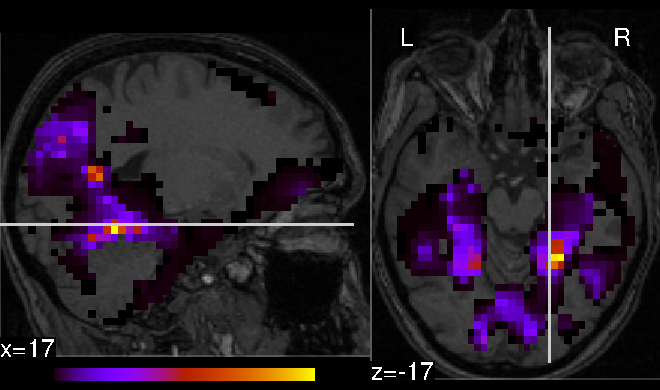
\includegraphics[width=.32\linewidth]{maps/face_vs_house_tol_0_1.pdf}%
                                    \llap{\color{white}\raisebox{.17\linewidth}{\rlap{\sffamily Stopping:
                                          $\Delta E < 10^{-1}$}}\hspace*{.315\linewidth}}\hfill%
                                    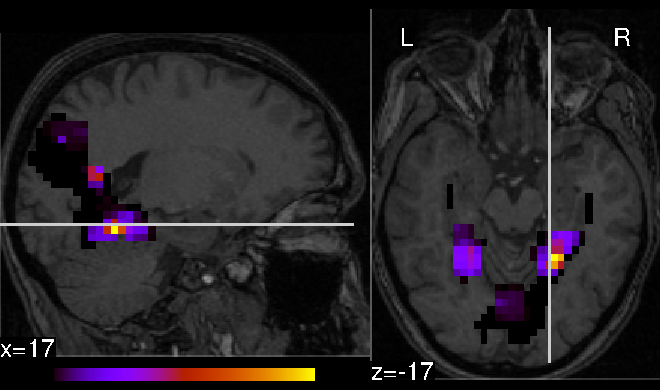
\includegraphics[width=.32\linewidth]{maps/face_vs_house_tol_0_001.pdf}%
                                    \llap{\color{white}\raisebox{.17\linewidth}{\rlap{\sffamily Stopping:
                                          $\Delta E < 10^{-3}$}}\hspace*{.315\linewidth}}\hfill%
                                    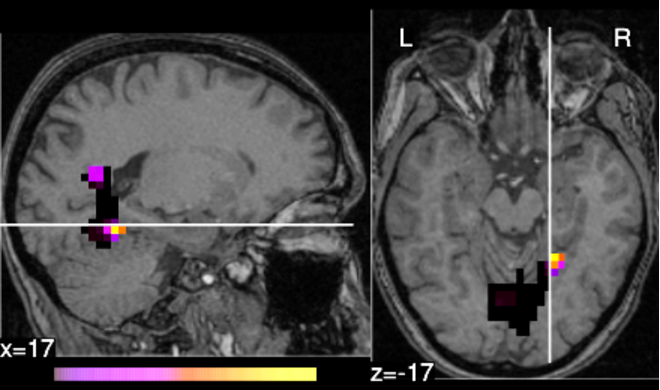
\includegraphics[width=.32\linewidth]{maps/face_vs_house_tol_1e-05.pdf}%
                                    \llap{\color{white}\raisebox{.17\linewidth}{\rlap{\sffamily Stopping:
                                          $\Delta E < 10^{-5}$}}\hspace*{.315\linewidth}}%
                                    \caption{TV$-\ell_1$ maps ($\hat{w}$) for the face-house discrimination task on
                                      the HAXBY2001 dataset, for different levels of \textcolor{orange}{tolerance}.
                                      This figure shows the importance of convergence for problem \eqref{eq:opt_pb}, and motivates
                                      the need for a fast solver.}%
                                    \label{fig:maps_tolerance}
                                  \end{figure}

                                  \end{nbox}
			\end{column}
			\hfill
			\begin{column}{.48\linewidth}
			  \begin{nbox}[\textwidth]{\textbf{Benchmarks (only TV-$\ell_1$)}}                          
                            \begin{figure}
                              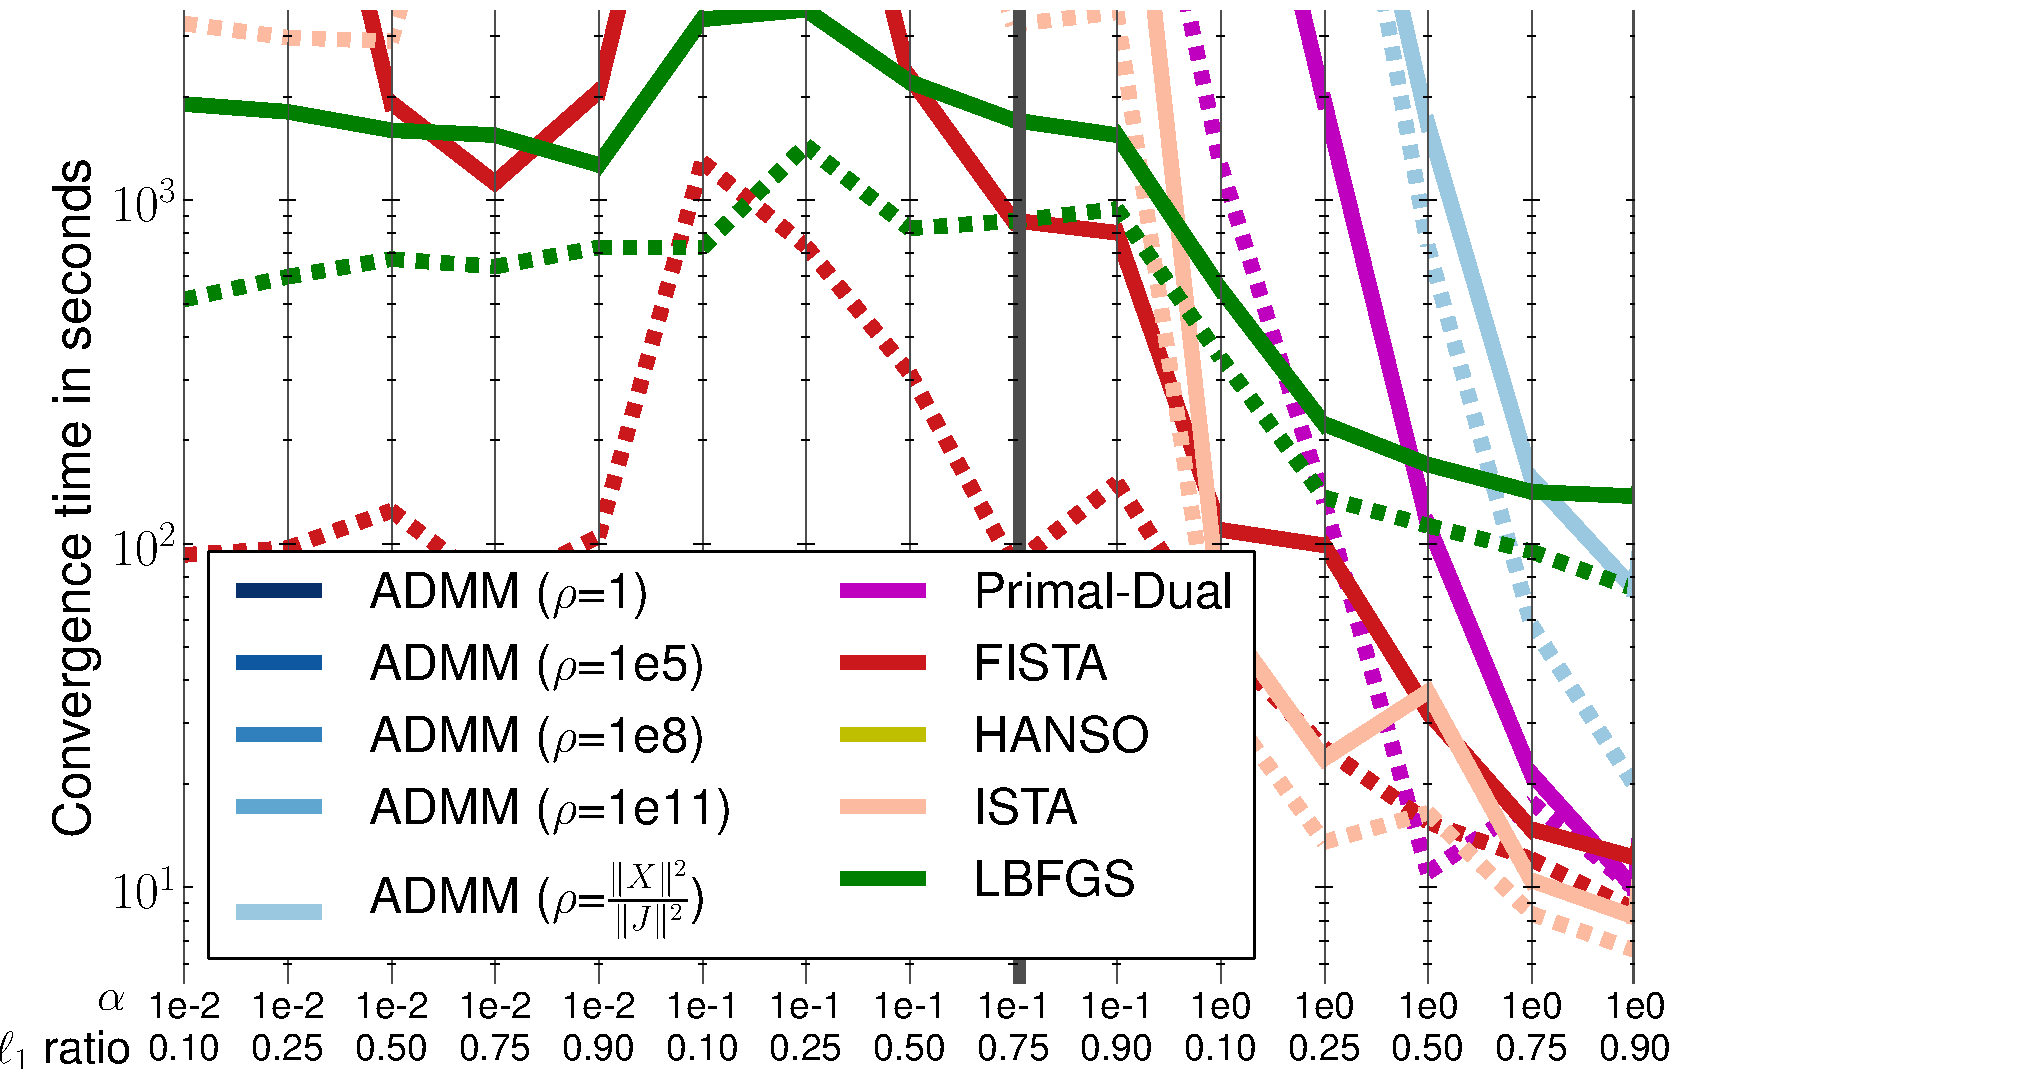
\includegraphics[width=1.2\linewidth]{bench/haxby_mse.pdf}%
                              \hspace{-.09\linewidth}%
                              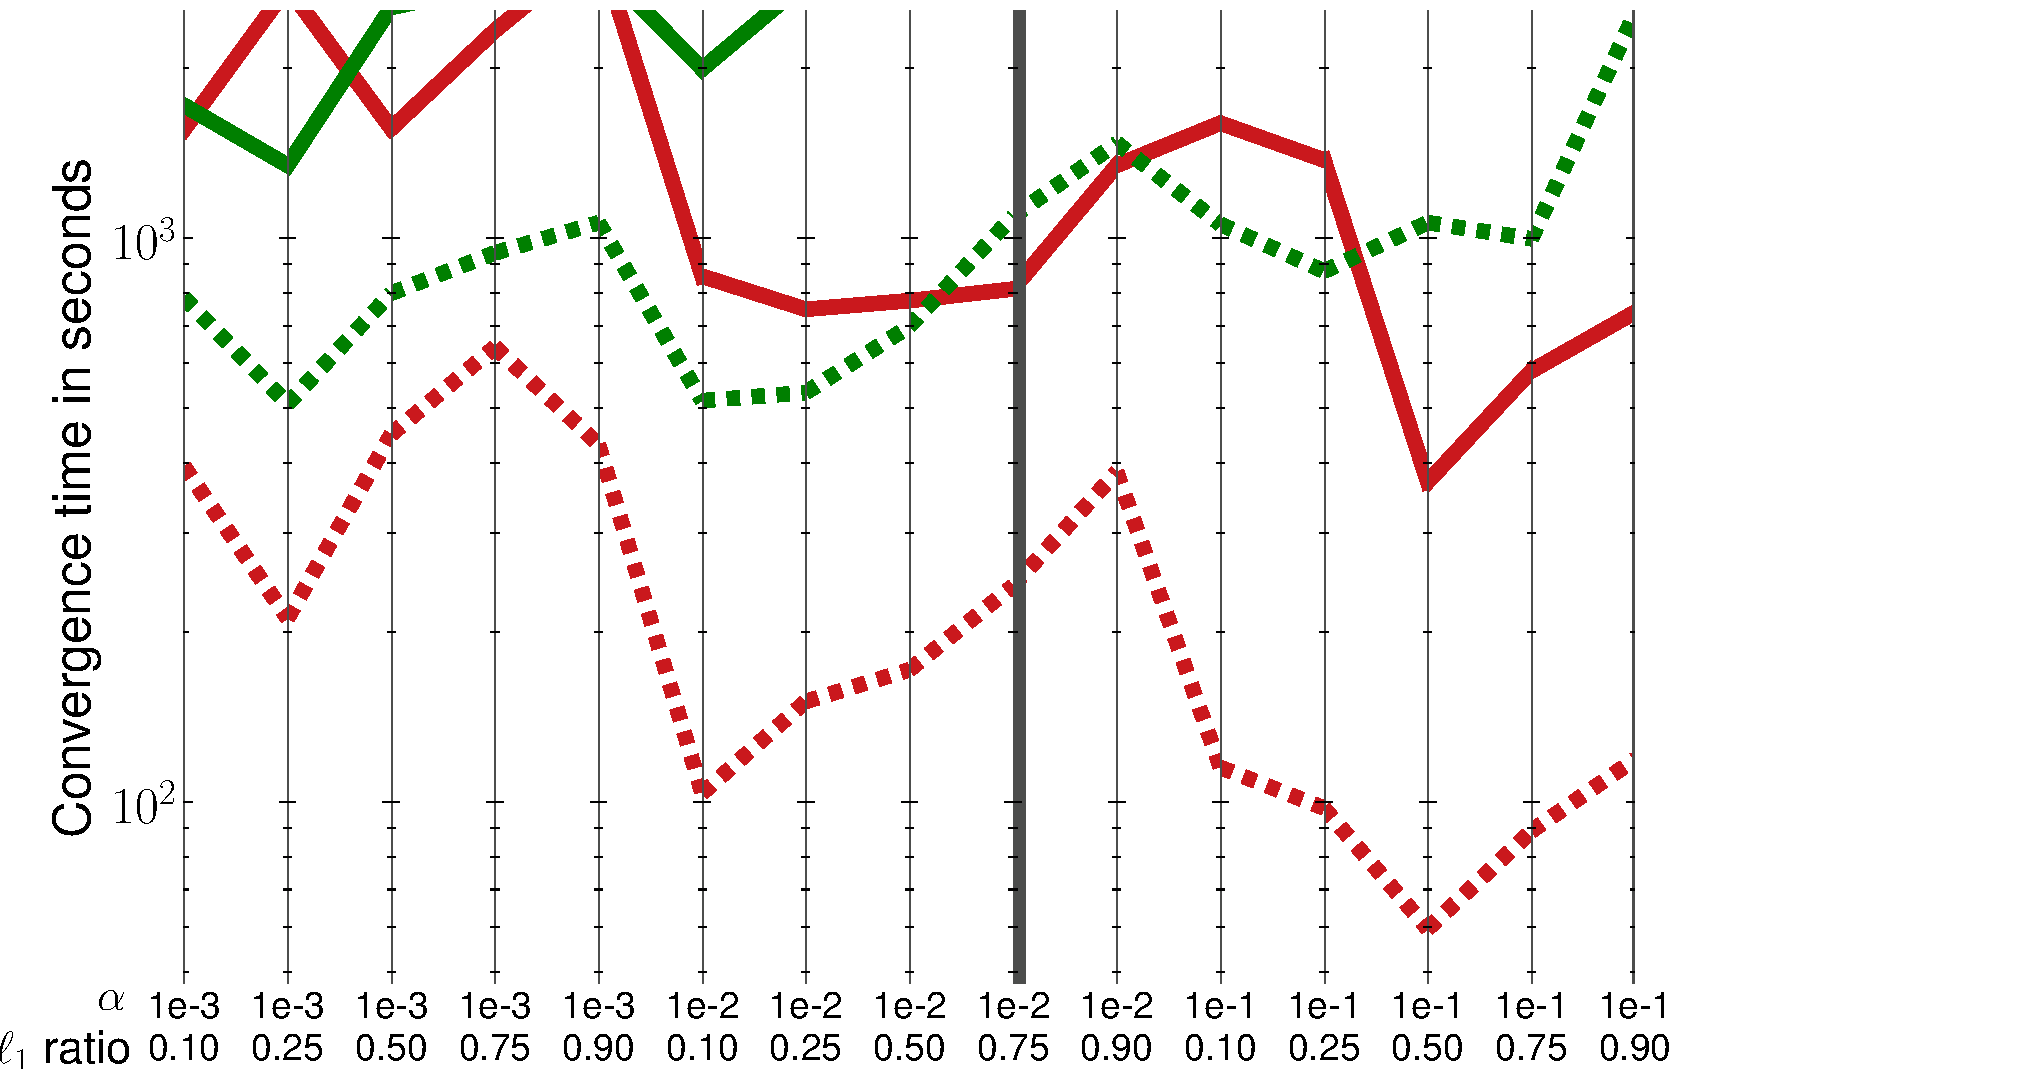
\includegraphics[width=1.2\linewidth]{bench/poldrack_mse.pdf}
                              \caption{TV$-\ell_1$ penalized Least-Squares Regression. \textbf{Top}:
                                on the visual recognition  face-house discrimination task; \textbf{Bottom}: on the
                                Mixed gambles dataset. Broken lines correspond to a tolerance of $10^{0}$,
                                whilst full-lines correspond to $10^{-2}$. The thick vertical line
                                indicates the best model selected by cross-validation.}
                              \label{Fig:MSEtimes}
                            \end{figure}
					%% Ce template a été fait sur la base du Template Beamer, vous retrouverez des fonctionnalités communes comme par exemple :
					%% \begin{itemize}
					%% 	\item Exemple d'item
					%% 	\begin{itemize}
					%% 		\item Exemple de sous-item
					%% 		\begin{itemize}
					%% 			\item Exemple de sous-sous-item
					%% 		\end{itemize}
					%% 	\end{itemize}
					%% 	\item Quelques fonctions disponibles avec le package : 
					%% \end{itemize}
					%% \Atext{Exemple de texte mis en évidence}{.5\textwidth}
					%% \Atext{Exemple de texte mis en évidence. On peut modifier la largeur de la boîte}{.9\textwidth}
					%% et une barre de progression \myprogressbar{30} avec différentes options \myprogressbar[scale=.4]{70}\\
					%% \vspace{.3cm}
				\end{nbox}
			\end{column}
			\hfill
		\end{columns}
	\end{frame}

\bibliographystyle{IEEEtran} \bibliography{IEEEabrv,bib_tv}
\end{document}
